\documentclass[11pt,a4paper]{ctexart}
\usepackage{fontspec}
\defaultfontfeatures{Mapping=tex-text}
\usepackage{xunicode}
\usepackage{xltxtra}
%\setmainfont{???}
\usepackage{amsmath}
\usepackage{amsfonts}
\usepackage{amssymb}
\usepackage{graphicx}
\usepackage{amsthm}
\usepackage{array}
\usepackage{float}   %{H}
\usepackage{booktabs}  %\toprule[1.5pt]
\usepackage[titletoc]{appendix}
\usepackage{tcolorbox} %彩色框框
%===================%插入代码需要的控制
\usepackage{listings}
\usepackage{xcolor}
\setmonofont{Consolas}%字体
\lstset{
	numbers=left, 
	numberstyle= \tiny, 
	keywordstyle= \color{ blue!70},
	commentstyle= \color{red!50!green!50!blue!50}, 
	frame=shadowbox, % 阴影效果
	rulesepcolor= \color{ red!20!green!20!blue!20} ,
	escapeinside=``,% 英文分号中可写入中文
	breaklines=true,
	basicstyle=\ttfamily 
} 
%===================%
\usepackage[left=2cm,right=2cm,top=2cm,bottom=2cm]{geometry}

\newtheorem{theorem}{定理}
\newtheorem{definition}{定义}
\newtheorem*{solution}{解}

\title{定性数据统计分析作业 (4)}
\author{钟瑜 \quad 222018314210044}
\date{\today}
\begin{document}
\maketitle
\pagestyle{plain}%设置页码
%==================================================================================%
\begin{figure}[H]
	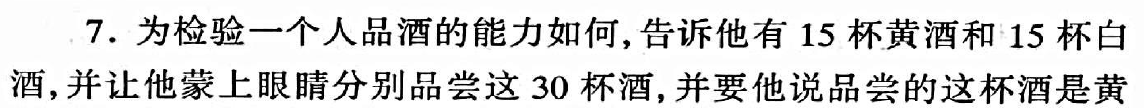
\includegraphics[width=0.7\textwidth]{screenshot001}
\end{figure}
\begin{figure}[H]
	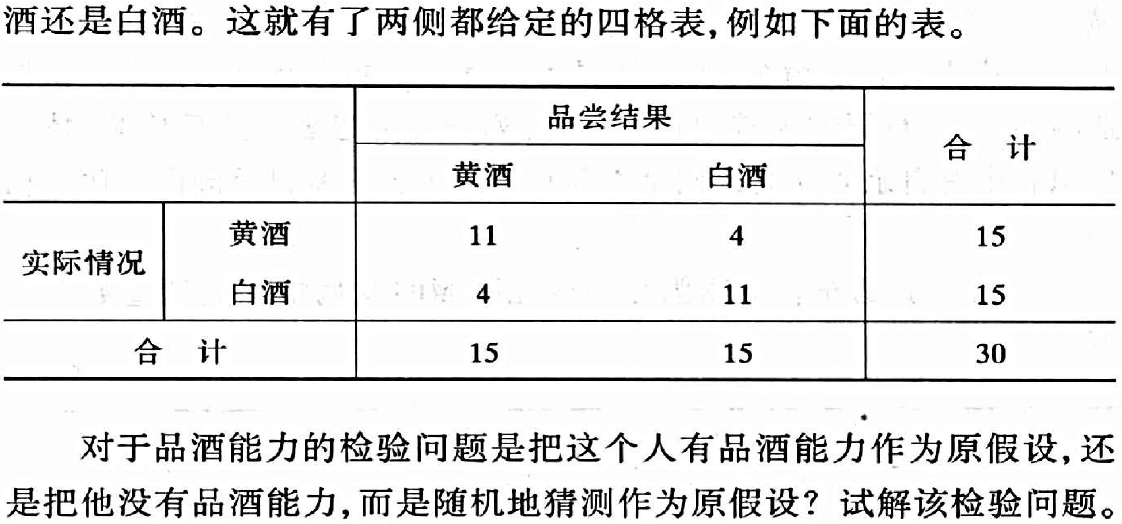
\includegraphics[width=0.7\textwidth]{screenshot002}
\end{figure}

\begin{solution}
\end{solution}

\begin{lstlisting}[language=r]
> x<-matrix(c(11,4,4,11),nrow=2) 
> fisher.test(x,alternative = "greater")

Fisher's Exact Test for Count Data

data:  x
p-value = 0.01342
alternative hypothesis: true odds ratio is greater than 1
95 percent confidence interval:
1.500179      Inf
sample estimates:
odds ratio 
6.983892 
\end{lstlisting}
p值大于$ \alpha $=0.01,故接受原假设,认为有品酒能力.\\

\begin{figure}[H]
	
\includegraphics[width=0.7\textwidth]{screenshot003}
\end{figure}
\begin{solution}
\end{solution}
\begin{lstlisting}[language=r]
> x<-matrix(c(28,9,18,17),nrow=2) 
> mcnemar.test(x,correct=F)

McNemar's Chi-squared test with continuity correction

data:  x
McNemar's chi-squared = 2.3704, df = 1, p-value = 0.1237
\end{lstlisting}
p值大于$ \alpha $=0.01,故接受原假设,认为比例相同.\\

\begin{figure}[H]
	
\includegraphics[width=0.7\textwidth]{screenshot004}
\end{figure}
\begin{solution}
	四格表如下所示:
	\begin{table}[!htbp]   %[H]
		\centering
		\begin{tabular}{cccc}
			\toprule[1.5pt]
			& 24  & 6 & 合计\\
			\midrule[1pt]
			买& 4 & 31 & 35\\
			不买 & 238 & 229 & 467\\
			\midrule[1pt]
			合计 & 242 & 260 & 502\\
			\bottomrule[1.5pt]
		\end{tabular}
	\end{table}
\end{solution}
\begin{lstlisting}[language=r]
> x<-matrix(c(4,31,238,229),nrow=2)
> fisher.test(x)

Fisher's Exact Test for Count Data

data:  x
p-value = 4.408e-06
alternative hypothesis: true odds ratio is not equal to 1
95 percent confidence interval:
0.03146334 0.36030504
sample estimates:
odds ratio 
0.1245649 
\end{lstlisting}
p值大于$ \alpha $=0.01,故拒绝原假设,认为选择多一些和少一些有显著差异.\\
\end{document}